\documentclass[11pt,landscape,a4paper,fleqn]{article}
\usepackage[dvipsnames]{xcolor} 
% https://www.overleaf.com/learn/latex/Using_colours_in_LaTeX#Reference_guide
\usepackage[utf8]{inputenc}
\usepackage[ngerman]{babel}
\usepackage{tikz}
\usetikzlibrary{shapes,positioning,arrows,fit,calc,graphs,graphs.standard}
\usepackage[nosf]{kpfonts}
\usepackage[vlined]{algorithm2e}
\usepackage[t1]{sourcesanspro}
%\usepackage[lf]{MyriadPro}
%\usepackage[lf,minionint]{MinionPro}
\usepackage{multicol}
\usepackage{wrapfig}
\usepackage[top=0mm,bottom=3mm,left=1mm,right=1mm]{geometry}
\usepackage[framemethod=tikz]{mdframed}
\usepackage{microtype}
\usepackage{soul}


\let\bar\overline

\definecolor{myblue}{cmyk}{1,.72,0,.38}
% \definecolor{myorange}{cmyk}{0,0.5,1,0}

\pgfdeclarelayer{background}
\pgfsetlayers{background,main}

\everymath\expandafter{\the\everymath \color{myblue}}
\everydisplay\expandafter{\the\everydisplay \color{myblue}}

\renewcommand{\baselinestretch}{.8}
\pagestyle{empty}

\global\mdfdefinestyle{header}{%
linecolor=gray,linewidth=1pt,%
leftmargin=0mm,rightmargin=0mm,skipbelow=0mm,skipabove=0mm,
}

\newcommand{\header}{
\begin{mdframed}[style=header]
\footnotesize
\sffamily
Cheat sheet\\
Ines Pereira,~page~\thepage~of~2
\end{mdframed}
}

\makeatletter
\renewcommand{\section}{\@startsection{section}{1}{0mm}%
                                {.2ex}%
                                {.2ex}%x
                                {\color{Maroon}\sffamily\small\bfseries}}
\renewcommand{\subsection}{\@startsection{subsection}{1}{0mm}%
                                {.2ex}%
                                {.2ex}%x
                                {\color{OliveGreen}\sffamily\bfseries}}
\renewcommand{\subsubsection}{\@startsection{subsubsection}{1}{0mm}%
                                {.2ex}%
                                {.2ex}%x
                                {\color{Black}\sffamily\bfseries}}

                                \DeclareMathOperator*{\argmin}{arg\,min}
                                \DeclareMathOperator*{\argmax}{arg\,max}

\makeatother
\setlength{\parindent}{0pt}

\newcommand\mycommfont[1]{\scriptsize\ttfamily\textcolor{blue}{#1}}
\SetCommentSty{mycommfont}

\begin{document}
\small
\begin{multicols*}{4}
    \section{Review of useful concepts and Introduction}
\subsection{Multivariate Gaussian}
%$\sigma =$ covariance matrix, $\mu$ = mean\\
$f(x) = \frac{1}{2\pi \sqrt{|\Sigma|}} e^{- \frac{1}{2} (x-\mu)^T \Sigma^{-1} (x-\mu)}$

Suppose we have a Gaussian random vector $X_V \sim N(\mu_V, \Sigma_{VV})$.\\
Suppose we take two disjoint subsets of V: $A={i_1,...,i_k}$ and $B={j_1,...,j_m}$.\\
Then, the conditional distribution: \\
$P(X_A|X_B=x_B)=N(\mu_{A|B}, \Sigma_{A|B})$ is Gaussian:\\
$\mu_{A|B}=\mu_A+\Sigma_{AB}\Sigma^{-1}_{BB}(x_B-\mu_B)$\\
$\Sigma_{A|B}=\Sigma_{AA}-\Sigma_{AB}\Sigma^{-1}_{BB}\Sigma_{BA}$

\subsection{Convex / Jensen's inequality}
$\text{g(x) is convex} \Leftrightarrow x_1,x_2 \in \mathbb{R}, \lambda \in [0,1]: g''(x) > 0$\\
$g(\lambda x_1 + (1-\lambda) x_2) \leq \lambda g(x_1) + (1-\lambda) g(x_2)$
$\varphi(\operatorname{E}[X]) \leq  \operatorname{E}[\varphi(X)]$
\subsection{Kullback-Leiber divergence}
$KL(p\vert\vert q)=\mathbb{E}_p\left[\log\frac{p(x)}{q(x)}\right]$\\
if $p_0\sim \mathcal{N}(\mu_0,\Sigma_0),\; p_1\sim \mathcal{N}(\mu_1,\Sigma_1) \Rightarrow KL(p_0\vert\vert p_1)$\\
{\scriptsize$ = \frac{1}{2}\left(tr\left(\Sigma_1^{-1}\Sigma_0\right) + (\mu_1-\mu_0)^T\Sigma_1^{-1}(\mu_1-\mu_0)-k+\log\frac{\vert\Sigma_1\vert}{\vert\Sigma_0\vert}\right)$}\\
$\hat q = \argmin_q KL(p\vert\vert q) \Rightarrow$ overconservative\\
$\hat q = \argmin_q KL(q\vert\vert p) \Rightarrow$ overconfident

    \section{Bayesian Regression}
$w\sim N(0,\sigma_p^2I),\;\epsilon \sim N(0,\sigma_n^2I),\; y=Xw+\epsilon$\\
$y\vert w \sim N(Xw,\sigma_n^2I)$\\
$w\vert y \sim N({(X^TX+\lambda I)}^{-1}X^Ty, {(X^TX+\lambda I)}^{-1}\sigma_n^2)$
    \section{Kalman Filter}
\(
\begin{cases}
    X_{t+1} = FX_t + \epsilon_t & \epsilon_t\sim N(0,\Sigma_x)\\
    Y_t=HX_t+\eta_t & \eta_t \sim N(0,\Sigma_y)\\
\end{cases} {X_1\sim N(\mu_p, \Sigma_p)}
\)
Then if $X_0$ is Gaussian then $X_{t}\vert Y_{1:t} \sim N(\mu_t, \sigma_t)$:\\
$\mu_{t+1} =F\mu_t+K_{t+1}(y_{t+1}-HF\mu_t)$\\
$\Sigma_{t+1}=(I-K_{t+1}H)(F\Sigma_tF^T+\Sigma_x)$\\
$K_{t+1} = ${\scriptsize $(F\Sigma_tF^T +\Sigma_x)H^T{(H(F\Sigma_tF^T+\Sigma_x)H^T+\Sigma_y)}^{-1}$}

    % -*- root: Main.tex -*-
\section{Gaussian Processes}
$f\sim GP(\mu,k)\Rightarrow\forall \left\{x_1, \dots, x_n\right\} \,\forall n < \infty$\\
$\left[f(x_1)\dots f(x_n)\right]\sim N(\left[\mu(x_1)\dots \mu(x_n)\right], K)$\\ where $K_{ij}=k(x_i,x_j)$
% A GP $\{X_t\}_t$ is a collection of random variables from which any finite sample has a joint Gaussian distribution.\\
% For any finite set of points $T=\{t_1, \dots, t_n\}$ from a GP, it hold that $(X_{t_1}, \dots,X_{t_n})\sim \mathcal{N}(\pmb{\mu_T},\pmb{\Sigma_T})$ with $\pmb{\mu_T} = (\mu(t_1),\dots,\mu(t_n))$, $\pmb{\Sigma_T}(i,j)=k(X_{t_i},X_{t_j})$
\subsection{Gaussian Process Regression}
$f\sim GP(\mu,k)$ then: $f\vert y_{1:n},x_{1:n} \sim GP(\tilde{\mu},\tilde{k})$\\
$\tilde{\mu}(x) = \mu(x) + K_{A, x}^T{(K_{AA}+\epsilon I_n)}^{-1}\left(y_A-\mu_A\right)$\\
$\tilde{k}(x,x') = k(x,x') - K_{A,x}^T{(K_{AA}+\epsilon I_n)}^{-1} K_{A,x'}$\\
Where: $K_{A,x} = {\left[k(x_1,x)\dots k(x_n,x)\right]}^T$\\
${\left[K_{AA}\right]}_{ij} = k(x_i, x_j)$ and $\mu_A = {\left[\mu(x_1 \dots x_n)\right]}^T$\\


\subsection{Kernels}
	$k(x,y)$ is a kernel if it's symmetric semidefinite positive:\\
	$\forall \left\{x_1, \dots, x_n \right\}$ then for the Gram Matrix \\
	${\left[K\right]}_{ij}=k(x_i,x_j)$ holds $c^TKc\geq0\forall c$\\
    \textbf{Some Kernels:} (h is the bandwidth hyperp.)\\
    Gaussian (rbf): $k(x,y) = \exp( -\tfrac{||x-y||^2}{h^2})$\\
    Exponential: $k(x,y) = \exp( -\tfrac{||x-y||}{h})$\\
    Linear kernel: $k(x,y) = x^Ty$ (here $K_{AA} = XX^T$)\\
\subsection{Optimization of Kernel Parameters}
Given a dataset $A$, a kernel function $k(x,y;\theta)$. $y\sim N(0, K_y(\theta))$ where $K_y(\theta)=K_{AA}(\theta)+\sigma_n^2I$\\
$\hat\theta = \argmax_\theta \log p(y\vert X;\theta)$\\ 
In GP: $\hat\theta=\argmin_\theta y^TK_{y}^{-1}(\theta)y + \log\vert K_y(\theta)\vert$\\
We can from here $\nabla\downarrow$:\\
$\nabla_\theta \log p(y\vert X;\theta) = ${\scriptsize$\frac{1}{2}tr\left(\left(\alpha\alpha^T-K^{-1}\right)\frac{\partial K}{\partial \theta}\right)$, $\alpha = K^{-1}y$}\\
Or we could also be baysian about $\theta$
\subsection{Aproximation Techniques}
\textbf{Local method:} $k(x_1,x_2)= 0$ if $||x_1-x_2||>\!\!>1$\\
\textbf{Random Fourier Features:} if $k(x,y)=\kappa(x-y)$\\
$p(w)=\mathcal{F}\left\{\kappa(\cdot), w\right\}$. Then $p(w)$ can be normalized to be a density.\\
$\kappa(x-y) = \mathbb{E}_{p(w)}\left[\exp{\left\{iw^T(x-y)\right\}}\right]$ {\scriptsize antitransform}\\
$\kappa(x-y) = \mathbb{E}_{b\sim \mathcal{U}(\left[0, 2\pi\right]), w\sim p(w)}\left[z_{w,b}(x)z_{w,b}(y)\right]$\\
where $z_{w,b}(x)=\sqrt{2}cos(w^Tx+b)$. I can MC extract features $z$. If \# features is $<\!\!<$ n then this is faster ($X^TX$ vs $XX^T$)\\
\textbf{Inducing points:} We a vector of inducing variables $u$\\
$f_A\vert_u \sim N(K_{Au}K_uu^{-1}u, \begingroup\color{magenta}K_{AA}-K_{Au}K_uu^{-1}K_{uA} \endgroup)$\\
$f_*\vert_u \sim N(K_{*u}K_uu^{-1}u, \begingroup\color{magenta}K_{**}-K_{*u}K_uu^{-1}K_{u*} \endgroup)$\\
\textbf{Subset of Regressors (SoR):} $\begingroup\color{magenta}\blacksquare\endgroup  \to 0$\\
\textbf{FITC:} $\begingroup\color{magenta}\blacksquare\endgroup  \to$ its diagonal\\
 
    
\section{Approximate inference}


\subsection{Laplace Approximation}
$\hat\theta=\argmax_\theta p(\theta\vert y)$\\
$\Lambda = -\nabla_\theta \nabla_\theta \log{p(\theta\vert y)}\vert_{\theta = \hat\theta}$\\
$p(\theta\vert y)\simeq q(\theta)=N(\hat\theta,\Lambda^{-1})$


\subsection{Variationa Inverence}
$\hat q = \argmin_{q \in Q} KL(q\vert\vert p(\cdot\vert y))$\\
$\hat q = \argmax_{q \in Q} ELBO$ Evidence Lower Bound\\
$ELBO \doteq \mathbb{E}_{\theta \sim q}\left[\log{p(y\vert\theta)}\right]-KL(q\vert\vert p(\cdot)) \leq \log{p(y)}$


\subsection{Markov Chain Monte Carlo}
\textbf{Idea}: All we need is sampling from postirior

\textbf{Ergodic Markov Chain}: \\
$\exists t \text{ s.t. } \mathbb{P}(i \to j \text{ in t steps})>0\;\; \forall i,j \Rightarrow\\
 \exists! \pi = \lim_{N\to \infty} \mathbb{P}(X_n=x)$ Limit distribution\\

 \textbf{Ergodic Theorem}: if $(X_i)_{i\in\mathbb{N}}$ is ergodic:\\
$\ \lim_{N\to \infty}\frac{1}{n}\sum_{i=1}^{N}f(X_i)=\mathbb{E}_{x\sim\pi}\left[f(x)\right]$\\

\textbf{Detailed Blanced Equation}:\\
$P(x\vert x')$ is the transition model of a MC:\\
if $R(x)P(x'\vert x) = R(x')P(x\vert x')$ then $R$ is the limit distribution of the MC \\

\textbf{Metropolis Hastings Algo}: Sample from a MC which has $P(x) = \frac{Q(x)}{Z}$ as limit dist.\\
\begin{algorithm}[H]
    \SetKwFor{kwWith}{with}{do}{}
    \SetKwInput{kwInit}{init}
    \KwResult{$\left\{X_i\right\}_{i\in\mathbb{N}}$ sampled from the MC}
    \kwInit{ $R(x\vert x')$ }
    \tcc{Good $R$ choice $\to$ fast convergence} 
    \kwInit{ $X_0 = x_0$ }
    \For{$t \gets 1, 2, \dots$}{
        $x' \sim R(\cdot, x_{t-1})$\\
        $\alpha = \min\left\{1;\frac{Q(x')R(x_{t-1}\vert x')}{Q(x_{t-1})R(x'\vert x_{t-1})}\right\}$\\
        \kwWith{probability  $\alpha$}
        {
            $X_{t} = x'$\;
        }
        otherwise $X_{t} = x_{t-1}$\;
     }
 \end{algorithm}
\textbf{Metropolis Adj. Langevin Algo (MALA)}:\\
Energy function: $P(x)=\frac{Q(x)}{Z}=\frac{1}{Z}\exp{(-f(x))}$\\
We chose: $R(x\vert x') = \mathcal{N}(x' - \tau \nabla f(x), 2\tau I)$\\
\textbf{Stoch. Grad. Langevin Dynamics (SGLD)}:\\
We use SGD to Approximate $\nabla f$. Converges also without acceptance step \\
\textbf{Hamilton MC}: SGD performance improoved by adding momentum (consider last step $\nabla f$)
\textbf{Gibbs sampling}: Practical when $X\in\mathbb{R}^n$\\
Used when $P(X_{1:n})$ is hard but $P(X_i\vert X_{-i})$ is easy.
\begin{algorithm}[H]
    \SetKwInput{kwInit}{init}
    \SetKwFor{kwWith}{with}{do}{}
    \kwInit{$x_0 \in \mathbb{R}^n;\; (x_0^{(B)} = x^{(B)})$ B is our data}
    \For {$t = 1,2,\dots$}
    {
        $x_t = x_{t-1}$\\

        \kwWith{ $i \sim \mathcal{U}(\left\{1:n\right\}\setminus B)*$}{
        $x_{t-1}^{(i)}\sim P(x^{(i)}\vert x^{(-i)})$
        }
    }
\end{algorithm}
$*$ if we do it $\forall i \notin B$ no DBE but more practical


\subsection{Variable elimination for MPE (most probable explanation):}
With loopy graphs, BP is often \textbf{overconfident/oscillates}.

\iffalse
- Given BN and evidence E=e\\
- Choose an ordering of $X_1, ... x_n$\\
- Set up initial factors $f_i=P(X_i|Pa_i)$\\
- For $i=1:n, X_i \notin  E$:\\
$\quad$ - Collect and multiply all factors $f_j$ that include $X_i$\\
$\quad$ - Generate new factor by maximizing out $X_i$:
        $g_i=\underset{w=x_i}{\operatorname{max}}\prod_j f_j$\\
$\quad$ - Add $g$ to set of factors\\
- For $i=n-1:1, X_i\notin E$:
    $\hat{x}_i=\underset{x_i}{\operatorname{argmax}}g_i(x_i, \hat{x}_{i+1:n})$

\textbf{Retrieving MAP from Max-Product (MAP = MPE for a subset of RVs):}\\
- Define max-marginals:\\
    $P_{max}(X_v=x_v):=\underset{x\sim x_v}{\operatorname{max}}P(x)$\\
- For tree factor graphs, max-product computes max-marginals:\\
    $P_{max}(X_v=x_v)	\propto \prod_{u \in N(v)} \mu_{u \rightarrow v}(x_v)$\\
- Can retrieve MAP solution from these (must be careful when ties need to be broken).


\subsection{Sampling based inference: compute marginals as expectations}
\textbf{Hoeffding's inequality:} Suppose $f$ is bounded in $[0, C]$. Then:\\
$P(|E_P[f(X)]-\frac{1}{N}\sum_{i=1}^N f(x_i)|\geq\epsilon) \leq 2exp\big( \frac{-2N\epsilon^2}{C^2}\big)$

\textbf{Monte Carlo Sampling from a BN:}\\
- Sort variables in topological ordering $X_1, X_n$\\
- For $i=1$ to $n$, sample:\\
$x_i \sim P(X_1=x_1, ..., X_{i-1}=x_{i-1})$

\textbf{Rejection Sampling}:\\
- Collect samples over all variables:\\
    $\hat{P}(X_A =x+A | X_B=x_B)=\frac{Count(x_A, x_B)}{Count(x_B)}$\\
- Throw away samples that disagree with $x_B$\\
- Count fraction of $x_a$ on remaining samples


\subsubsection{Directly sampling from the posterior: MCMC}
\textbf{Markov Chain:}: A (stationary) MC is a sequence of RVs $X_1, ..., X_N$, with prior $P(X_1)$ and transition probabilities $P(X_{t+1}|X_t)$ independent of t.\\
\textbf{Markov assumpt.:} $X_{1:t-1}\perp X_{t+1:T}|X_t$, $\forall t>1$\\
\textbf{Stationarity assumption:}\\
$P(X_{t+1}=x|X_t=x')=P(X_{t}=x|X_{t-1}=x')$, $\forall t>1$\\
\textbf{If ergodic} (= there exists a finite t such that every state can be reached in exactly t steps), then: it has a unique and positive stationary distribution $\pi(X)>0$, such for all $x$:\\
            $\underset{N\rightarrow\infty}{lim}P(X_N=x)=\pi(x)$ and $\pi(X)\perp P(X_1)$.\\
If MC satisfies the \textbf{detailed balance equation} (for unnormalized distribution $Q$, for all $x,x'$: $Q(x)P(x'|x)=Q(x')P(x|x')$), then the MC has stationarity distribution $\pi(X)=1/ZQ(X)$.

\textbf{Designing Markov Chains:}\\
- Proposal distribution $R(X'|X)$: given $X_t=x$, sample "proposal" $x'\sim R(X'|X=x)$\\
- Acceptance distribution\\
$\quad$ - Suppose $X_t=x$\\
$\quad$ - With probability $\alpha=min \Big\{1, \frac{Q(x')R(x|x')}{Q(x)R(x'|x)}\Big\}$
        set: $X_{t+1}=x'$\\
$\quad$ - With probability $1-\alpha$, set $X_{t+1}=x$\\

\textbf{MCMC for graphical models: Gibbs sampling (Random Vs \hl{Practical variant}):}\\
- Start with initial assignment $x$ to all variables\\
- Fix observed variables $X_B=x_B$\\
- For $t=1$ to $\infty$, do:\\
$\quad$ - Pick a variable $i$ uniformly at random from $\{1,...,n\}\setminus B$ \hl{/ Set ordering}, and then, for each $X_i$ (except those in $B$)\\
$\quad$ - Set $v_i=$ values of all $x$ except $x_i$\\
$\quad$ - Sample $x_i$ from $P(X_i|v_i)$
\fi




    \section{Bayesian Neural Nets}
Likelihood: $p(y\vert x;\theta) = \mathcal{N}(f_1(x,\theta), \exp{(f_2(x,\theta))})$\\
Prior: $p(\theta) = \mathcal{N}(0, \sigma_p^2)$\\
$\theta_{MAP} = \argmax \log{(p(y, \theta))}$

\subsection{Variation inference:} Usually we use $Q =$ Set of Gaussians\\
 $\hat q =  \argmax ELBO$ {\scriptsize Reparameterization trick}\\
$q$ approx. the posterior but how to predict?\\
$p(y^*\vert x^*, \mathcal{D})\simeq \frac{1}{m}\sum_{j=1}^m p(y^*\vert x^*, \theta^{(i)}),\;\theta \sim \hat q(\theta)$ \\
Gaussian Mixture distribution:
$\mathbb{V}(y^*\vert x^*,\mathcal{D}) \simeq \\
\simeq \begingroup\color{magenta}\frac{1}{m}\sum_{j=1}^m \sigma^2(x^*, \theta^{(i)})\endgroup + \begingroup\color{blue}\frac{1}{m}\sum_{j=1}^m\left(\mu(x^*,\theta^{(j)}-\bar\mu(x^*))\right)\endgroup$\\
$\begingroup\color{magenta}\blacksquare\endgroup \to $Aletoric,
$\begingroup\color{blue}\blacksquare\endgroup \to $Epistemic\\

\textbf{Dropouts Regularization}: Random ignore nodes in SGD iteration: 
Equavalent to VI with $Q = \left\{q(\cdot\vert \lambda) = \prod_j q_j(\theta_j\vert \lambda), \; \lambda \in \mathbb{R}^d \right\}$\\
where $q_j(\theta_j\vert \lambda) = p\delta_0(\theta_j) +  (1-p)\delta_{\lambda_j}(\theta_j)$\\
This allows to do Dropouts also in prediction

\subsection{MCMC:} MCMC but cannot store all the $\theta^{(i)}$:\\
1) Subsampling: Only store a subset of the  $\theta^{(i)}$\\
2) Gaussian Aproximation: We only keep:\\
$\mu_i=\frac{1}{T}\sum_{j=1}^T \theta_i^{(j)}$ and $\sigma_i=\frac{1}{T}\sum_{j=1}^T (\theta_i^{(j)}-\mu_i)^2$\\
And updete them online. 

\textbf{Predictive Esnable NNs}: \\
Let $\mathcal{D} = \left\{(x_i,y_i)\right\}_{i=1:n}$ be our dataset. \\
Train $\theta_i^{MAP}$ on $\mathcal{D}_i$ with $ i=1,\dots,m$\\
$\mathcal{D}_i$ is a Bootstrap of $\mathcal{D}$ of same size\\
and $p(y^*\vert x^*, \mathcal{D})\simeq \frac{1}{m}\sum_{j=1}^m p(y^*\vert x^*, \theta^{MAP}_i)$ 


\subsection{Model calibration}
Train $\hat q$ on $\mathcal{D}_{train}$ \\
Evaluate $\hat q$ on $\mathcal{D}_{val}= \left\{(y',x')\right\}_{i=1:m}$\\
Held-Out-Likelihood $\doteq \log{p(y'_{1:m} \vert x'_{1:m} , \mathcal{D}_{train})}$ \\
$\geq \mathbb{E}_{\theta \sim \hat q}\left[\sum_{i=1}^m\log{p(y_i'\vert x_i', \theta)}\right]$ (Jensen)\\
$\simeq \frac{1}{k}\sum_{j=1}^k\sum_{i=1}^m\log{p(y_i'\vert x_i', \theta^{(j)})}, \;\; \theta^{(j)} \sim \hat q$

\textbf{Evaluate predicted accuracy}: We divide $\mathcal{D}_{val}$ into bins according to predicted confidence values. In each bin we compare accuracy with confidence


    \section{Active Learning}
Let $\mathcal{D}$ be the set of observable points. \\
We can observe $\mathcal{S}\subseteq \mathcal{D}, \vert \mathcal{S}\vert\leq R$\\
Information Gain: $\hat{\mathcal{S}}=\argmax_{\mathcal{S}} F(\mathcal{S})=I(f,y_\mathcal{S})$\\
For GPs: $F(\mathcal{S})=\frac{1}{2}\log\left\lvert I+\frac{1}{\sigma^2}K_{\mathcal{SS}}\right\rvert $\\
This is NP Hard, $\Rightarrow$ Greedy Algo:\\
\begin{algorithm}[H]
    \SetKwInput{kwInit}{init}
    \SetKwFor{kwWith}{with}{do}{}
    \kwInit{$\mathcal{S}^*=\emptyset$}
    \For {$t = 1:R$}
    {
        $x_{t} = \argmax_{x\in\mathcal{D}}F(\mathcal{S^*}\cup\left\{x\right\})$\\
        $\left(x_{t} = \argmax_{x\in\mathcal{D}} \sigma^2_{x}\vert \mathcal{S}\text{ for GPs}\right)$\\
        $\left(x_{t} = \argmax_{x\in\mathcal{D}} \frac{\sigma^2_{f\vert \mathcal{S}}(x)}{\sigma^2_{n}(x)} \text{ for heter. GPs}\right)$\\
        $\mathcal{S^*} = \mathcal{S} \cup \left\{x_{t}\right\}$
    }
\end{algorithm}
F is \textbf{Submodular} if: $\forall x \in \mathcal{D}\;\;, \forall A \subseteq B \subseteq D$ holds that:
$F(A\cup\left\{x\right\})-F(A)\geq F(B\cup\left\{x\right\})-F(B)$\\
F is Submodular $\Rightarrow F(\mathcal{S}^*)\geq \left(1-\frac{1}{e}\right)F(\hat{\mathcal{S}})$

    \section{Bayesian Optimization}
Like Active Learning but we only want to find the optima. 
We pick $x_1, x_2, \dots$ from $\mathcal{D}$ and observe $y_i = f(x_t)+\epsilon_t$.\\
\textbf{Comulative regret:}$R_T=\sum\limits_{t=1}^T\left(\max_{x\in\mathcal{D}f(x) - f(x_t)}\right)$
\textbf{Oss:}$\frac{R_T}{T}\to 0 \Rightarrow \max_{t}f(x_t)\to \max_{x\in\mathcal{D}} f(x)$

\subsection{Upper Confidence Sampling}
With GP $x_t = \argmax_{x\in \mathcal{D}} \mu_{t-1}(x) + \beta_t \sigma_{t-1}(x)$\\
Chosing the correct $\beta_t$ we get: $\frac{R_T}{T}=\mathcal{O}\left(\sqrt{\frac{\gamma_T}{T}}\right)$.
Where $\gamma_t = \max_{|\mathcal{S}|<T}I(f;y_\mathcal{S})$. On d dims:\\
{\scriptsize Linear}: $\gamma_T=\mathcal{O}(d\log T)$ {\scriptsize RBF}: $\gamma_T=\mathcal{O}((log T)^{d+1})$\\
\textbf{Optimal $\beta_t$} $=\mathcal{O}(\left\lVert f\right\rVert_K^2+\gamma_t \log^3T )$\\
\textbf{Oss:} $\beta \uparrow = $more exploration
\subsection{Thompson Samling}
$x_t = \argmax_{x\in\mathcal{D}}\tilde{f}(x),\;\;\tilde{f}\sim p(f\vert x_{1:n}, y_{1:n})$


    \section{Markov Decision Process (MDP)}
\subsection{Definitions}
$\mathcal{X}=\left\{1,\dots,n\right\}$ states; 
$\mathcal{A}=\left\{1,\dots,m\right\}$ actions;\\
$p(x'\vert x, a)$ transition probability;\\
$r(x,a)$ reward {\tiny(can be random)}; 
$\pi:\mathcal{X}\rightarrow\mathcal{A}$ policy;\\
$T^\pi\in\mathbb{R}^{n\times n},\; T^\pi_{ij} = p(j\vert i, \pi(i))$ Transition Matrix:\\
$J(\pi) = \mathbb{E}\left[\sum_{i=0}^{\infty}\gamma^i r(X_i, \pi(X_i))\right]$ Expected value:\\
$V^\pi:\mathcal{X}\rightarrow \mathbb{R},\; x\mapsto J(\pi\vert X_0 = x)$ Value function;\\
$Q^V(x,a) = r(x,a) + \gamma\sum_{x\in\mathcal{X}}p(x'\vert x, a)V(x)$ Q func;\\
$\pi_\mathcal{G}^{V}(x)=\argmax_a Q^V(x,a)$ greedy policy {\scriptsize w.r.t. $V$};

\subsection{Value function Theorem}
$V^\pi(x) = r(x,\pi(x))+\gamma\sum_{x'\in\mathcal{X}}p(x'\vert x, \pi(x))V^\pi(x')$
Matrix formulation: $(I-\gamma T^\pi)V^\pi=r^\pi$

\subsection{Bellman Theorem}
1) $\pi^*$, $V^*$ are optimal policy and it's value func.\\
2) $\pi^* = \pi_\mathcal{G}^{V^*}$\\
3) $V^*(x)=max_a\left[r(x,a)+\gamma\sum_{x\in\mathcal{X}}p(x'\vert x, a)V^*(x)\right]$
1) $\Leftrightarrow$ 2) $\Leftrightarrow$ 3)

\subsection{Algorithms}
\subsubsection{Policy iteration}
\begin{algorithm}[H]
    \While(){no more changes}{
        $\pi \gets \pi_\mathcal{G}^{V}$ (Update the Policy)\\
        $V \gets (I-\gamma T^\pi)^{-1}r^\pi)$ (Update the value)
    }
\end{algorithm}

\subsubsection{Value iteration}
    \begin{algorithm}[H]
        \While(){$\left\lVert  V_t - V_{t-1}\right\rVert \leq \epsilon$}{
            \ForEach{$x\in \mathcal{X},\; a\in \mathcal{A}$}{
                $Q_t(x,a)\gets r(x,a)+\gamma \sum_{x'\in\mathcal{X}}p(x'\vert x, a)V_{t-1}(x)$\\
            }            
            \ForEach{$x\in \mathcal{X}$}{
                $V_t(x)\gets \max_a Q_t(x,a)$\\
            }
        }
        $\hat{\pi} = \pi_\mathcal{G}^{V_T}$; where $V_T$ last found Value
\end{algorithm}

\subsection{Partialy Observable MDP (POMDP)}
POMDP can be seen as MDP where:\\
1) $\mathcal{X}_{POMDP}$ are prob. distribution over $\mathcal{X}_{MDP}$\\
2) the actions are the same\\
3) $r_{POMDP}(b, a)= \mathbb{E}_{x\sim b}\left[r_{MDP}(x, a)\right]$\\
4) Trans. model: $b_{t+1}(x) = \mathbb{P}(X_{t+1}=x\vert y_{1:t+1}, a_t)$\\
$b_{t+1}(x) =${\scriptsize $\frac{1}{Z}p(y_{t+1}\vert X_{t+1}=x)\sum_{x'\in \mathcal{X}_{MDP}}p(x\vert x', a_t)b_t(x')$}
\textbf{How to solve?} Discretize $\mathcal{X}_{POMDP}$ and treat it as a MDP or Policy gradient techniques
    %\subsection{Review Probability}
\textbf{Probability space ($\Omega, F, P$):}
Set of atomic events $\Omega$.
Set of all non-atomic events ($\sigma$-Algebra): $F \in 2^{\Omega}$.
Probability measure: $P: F \rightarrow [0,1]$\\
\textbf{Bayes' rule}: $P(B|A)= P(A,B)/P(A)=P(A|B)P(B)/P(A)$, where $P(A)=\sum_bP(A|B)P(A)$
\textbf{Union:} $P(A\cup B)=P(A)+P(B)-P(A\cap B)$

% \textbf{Probability axioms:}\\
% Normalization\\
% Non-negativity\\
% $\sigma$-additivity

\textbf{Rules for joint distributions:}\\
Sum rule (Marginalization):\\
    $P(X_{1:i-1}, X_{i+1:n})=\sum_{x_i}P(X_{1:i-1}, X_i=x_i, X_{i+1:n})$
Product rule (Chain rule):\\
    $P(X_{1:n})=P(x_1)P(X_2|X_1)...P(X_n|X_{1:n-1})$

\textbf{Conditional Independence:}\\
$X\perp Y | Z $ iff $P(X,Y|Z)=P(X|Z)P(Y|Z)$\\
If $P(Y|Z)>0 \Rightarrow P(X|Z,Y)=P(X|Z)$ 

\textbf{Properties of Conditional Independence:}\\
Symmetry: $X \perp Y$ | $Z \Rightarrow Y \perp X$ | $Z$\\
Decomposition: $X \perp (Y,W)$ | $Z \Rightarrow X \perp Y$ | $Z$\\
Contraction: $(X \perp Y$ | $Z) \wedge (X \perp W$ | $Y, Z) \Rightarrow X \perp Y, W$ | $Z$\\
Weak union: $X \perp Y,W$ | $Z \Rightarrow X \perp Y$ | $Z, W$\\
Intersection: $(X \perp Y$ | $W, Z) \wedge (X \perp W$ | $Y, Z) \Rightarrow X \perp Y, W$ | $Z$

    %\section{Bayesian Networks}
\subsection{Basic concepts}
A Bayesian network ($G, P$) consists of:\\
- A BN structure $G$ (directed, acyclic graph)\\
- A set of conditional probability distributions\\
- ($G, P$) defines the joint distribution:\\
    $P(X_1, ..., X_n)=\prod_iP(X_i | Pa_{X_i})$

BNs with 3 nodes:

% 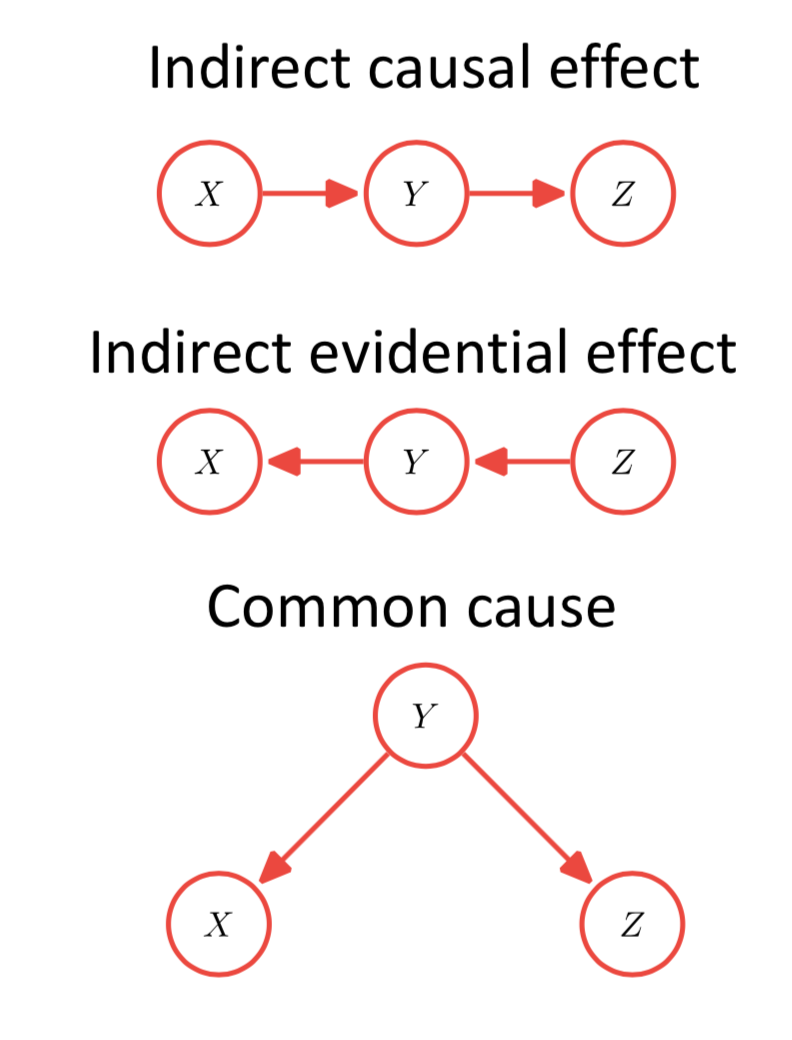
\includegraphics[scale=.2]{BN1.png}
% 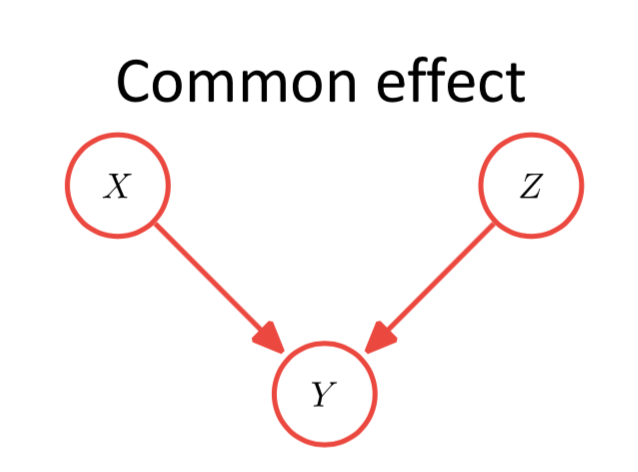
\includegraphics[scale=.2]{BN2.png}
\subsection{Active trails and d-separation}
An undirected path in a BN structure G is called active trail for observed variables $O \in {X_1, ..., X_n}$ of for every consecutive triple of variables X, Y, Z on the path:\\
- \textbf{indirect causal effect}:\\
$X \rightarrow Y \rightarrow Z$ and Y unobserved\\
- \textbf{indirect evidential effect}:\\
$X \leftarrow Y \leftarrow Z$ and Y unobserved\\
- \textbf{common cause}:\\
$X \leftarrow Y \rightarrow Z$ and Y unobserved.\\
- \textbf{common effect}:\\
$X \rightarrow Y \leftarrow Z$ and Y or any of Y's descendants is observed.\\
Any variables $X_i$ and $X_j$ for which there is no active trail for observations O are called d-separated by O.\\
\textbf{Theorem}: $d-sep(X_i;X_j|O)) \quad \Rightarrow X\perp Y |Z$\\
Converse does not hold in general!


    %\section{Exact inference (tree-structured BN) }
\subsection{Variable elimination}
- Given a BN and query $P(X|E=e)$\\
- Choose an ordering of $X_1, ..., X_n$ \textbf{Eliminate variables from the outside in!}\\
- Set up initial factors: $f_i=P(X_i|Pa_i)$\\
- For $i=1:n, X_i \notin {X, E}$\\
$\quad$ - Collect and multiply all factors $f$ that include $X_i$\\
$\quad$ - Generate new factor by marginalizing out $X_i$:
        ${g_X}_i = \sum_{x_i}\prod_j f_j$\\
$\quad$ - Add g to set of factors\\
- Renormalize $P(x,e)$ to get $P(x|e)$

\textbf{Variable elimination for polytrees:}\\
- Pick a root, (avoiding $X$ and $E$)\\
- Orient edges towards root\\
- Eliminate variables according to topological order


\subsection{Avoiding recomputation: factor graphs}
FG for a BN is a bipartite graph consisting of variables (circles) and factors (rectangles). \textbf{It is not a unique representation.}\\
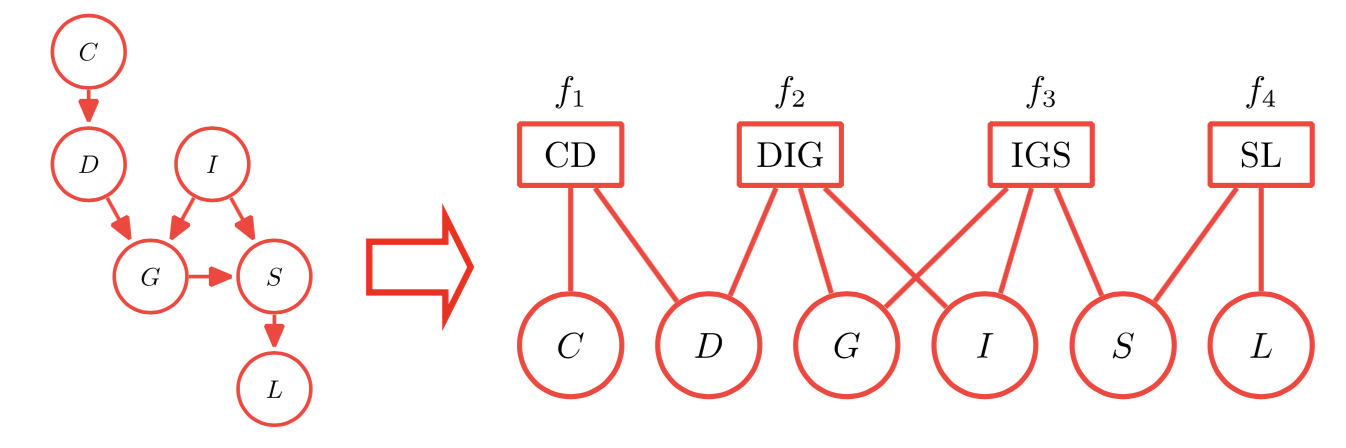
\includegraphics[scale=0.25]{images/factor_graph.png}
\subsubsection{Sum-product/Belief Propagation (BP) Algorithm:}
- Initialize all messages as uniform distribution\\
- Until converged to:\\
$\quad$ - Pick a root in the factor graph and reorient the edges towards this root.\\
$\quad$ -  Update messages according to this ordering. Do passes from leaves to root and from root to leaves.\\
- If a leaf node is a variable node: 
$\mu_{x\rightarrow f}(x)=1$
- If a leaf node is a factor node:
$\mu_{f \rightarrow x}(x)=f(x)$
- Messages from node $v$ to factor $u$:\\
    $\mu_{v\rightarrow u}(x_v) = \prod_{u'\in N(v)\setminus \{u\}}\mu_{u'\rightarrow v(x_v)}$\\
- Messages from factor $u$ to node $v$:\\
    $\mu_{u\rightarrow v}(x_v) = \sum_{x_u\sim x_v}f_u(x_u) \prod_{v'\in N(u)\setminus \{v\}}\mu_{v'\rightarrow u(x_v')}$
    % https://tex.stackexchange.com/questions/9363/how-does-one-insert-a-backslash-or-a-tilde-into-latex
$\quad$ -  Break once all messages change by $\leq \epsilon$

\textbf{Hope:} after convergence, we have:\\
$P(X_v=x_v)=\frac{1}{Z}\prod_{u \in N(v)}\mu_{u\rightarrow v}(x_v)$\\
$P(\overrightarrow{X_u}=\overrightarrow{x_u})=\frac{1}{Z} f_u(\overrightarrow{x_u})\prod_{v\in N(u)}\mu_{v\rightarrow u}(x_v)$

\textbf{If we have a polytree Bayesian network}:\\
- Choose one node as root\\
- Send messages from leaves to root and from root to leaves\\

    %\section{Dynamical models (include time)}

\subsection{Examples with one variable per time step}
% \textbf{Hidden Markov Models (HMM)}\\
% \textbf{Kalman FIlters}\\
% 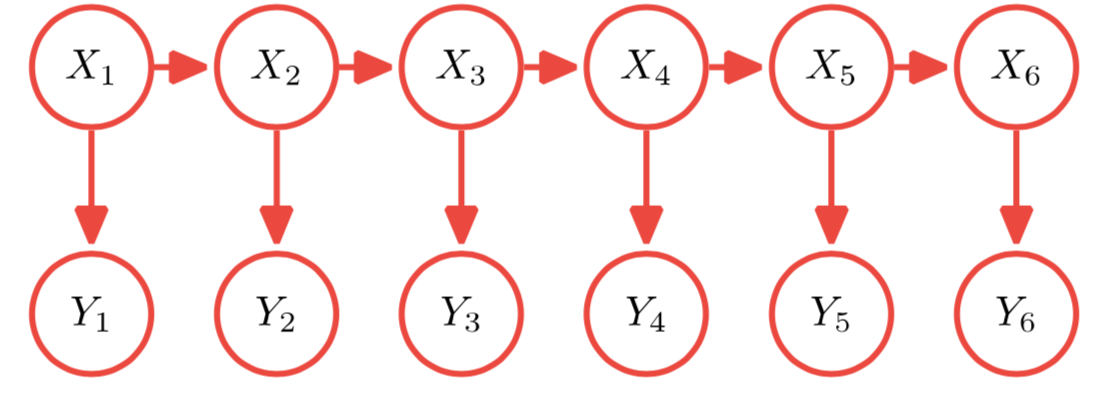
\includegraphics[scale=.25]{HMM_KF.png}\\
$X_1, ...,X_T$ (unobserved) hidden states\\
$Y_1, ...,Y_T$ (noisy) observations\\
\textbf{HMMs (polytrees: can use belief propagation):} $X_i$ categorical, $Y_i$ categorical (or arbitrary)\\
\textbf{Kalman filters:} $X_i, Y_i$ Gaussian distributions\\
- $P(X_1)$: prior belief about location at time i\\
- $P(X_{t+1}|X_t)$: \textbf{'Motion model'} (how do I expect my target to move in the environment?): 
    $X_{t+1}=FX + \epsilon_t$ where $\epsilon_t \sim N(0, \Sigma_x)$\\
- $P(Y_t|X_t)$: \textbf{'Sensor model'} (what do I observe if target is at location $X_t$?)
    $Y_t=HX_t+\eta_t$ where $\eta_t\sim N(0, \Sigma_y)$

\subsection{Inference tasks}
\textbf{Filtering}: $P(X_t|y_{1,...,t})$ Is it raining today?\\
\textbf{Prediction}: $P(X_{t+\tau}|Y_{1:t})$ Rain 5 days from now? \\
Example for one step:
$P(X_{t+1}|Y_{1:t})=\sum_x P(X_{t+1}, X_t=x_t|Y_{1:t})=\sum_x P(X_{t+1} | X_t=x_t)P(X_t|Y_{1:t})$ (with KFs, you need \textbf{integrals}!)\\
\textbf{Smoothing}: $P(X_\tau|y_{1:t})$ with $\tau<t$ Did it rain last week? [Can use sum-product (aka forward-backward).] \\
\textbf{MPE}:  $ \underset{x_{1:T}}{argmax}P(x_{1:T}|y_{1:T})$ Can use max product (aka Viterbi algorithm).\\
\textbf{Bayesian filtering:}
Start with $P(X_1)$:\\
At time t, assume we have $P(X_t|y_{1:t-1})$\\
Conditioning: 
$P(X_t|y_{1:t})= \frac{P(X_t|y_{1:t-1})P(y_t|X_t)}{\sum_{x_{t}} P(X_t|y_{1:t-1})P(y_t|X_t)}$\\
Prediction ($O(n^2)$ \textit{vs} $O(n)$ in conditioning):\\ 
$P(X_{t+1}|y_{1:t}) = \sum_x P(X_{t+1}|X_t)P(X_t|y_{1:t})$\\
\textbf{Since HMM is a polytree, smoothing/MPE can be computed by VE/BP.}
\textbf{Kalman filtering:} Bayesian filtering for continuous problems. RV corrupted by Gaussian distributions with zero mean. \textbf{Bayesian filtering is basically the same, except that sums turn to integrals.}
\textbf{General Kalman update}\\
- Transition model:
    $P(x_{t+1}|x_t)=N(x_{t+1};Fx_t, \Sigma_x)$\\
- Sensor model:
    $P(y_{t}|x_t)=N(y_{t};Hx_t, \Sigma_y)$\\
- Kalman update:\\
    $\mu_{t+1}=F\mu_t+K_{t+1}(y_{t+1}-HF\mu_t)$\\
    $\Sigma_{t+1}=(I-K_{t+1})(F\Sigma_tF^T + \Sigma_x)$\\
- Kalman gain:
    $K_{t+1}=(F\Sigma_t F^T+\Sigma_x)H^T(H(F\Sigma_t F^T+\Sigma_x)H^T+ \Sigma_y)^{-1}$


\subsection{Examples with > 1 variable per time step}
\textbf{Dynamic Bayesian Networks}: a BN at every time step\\
% 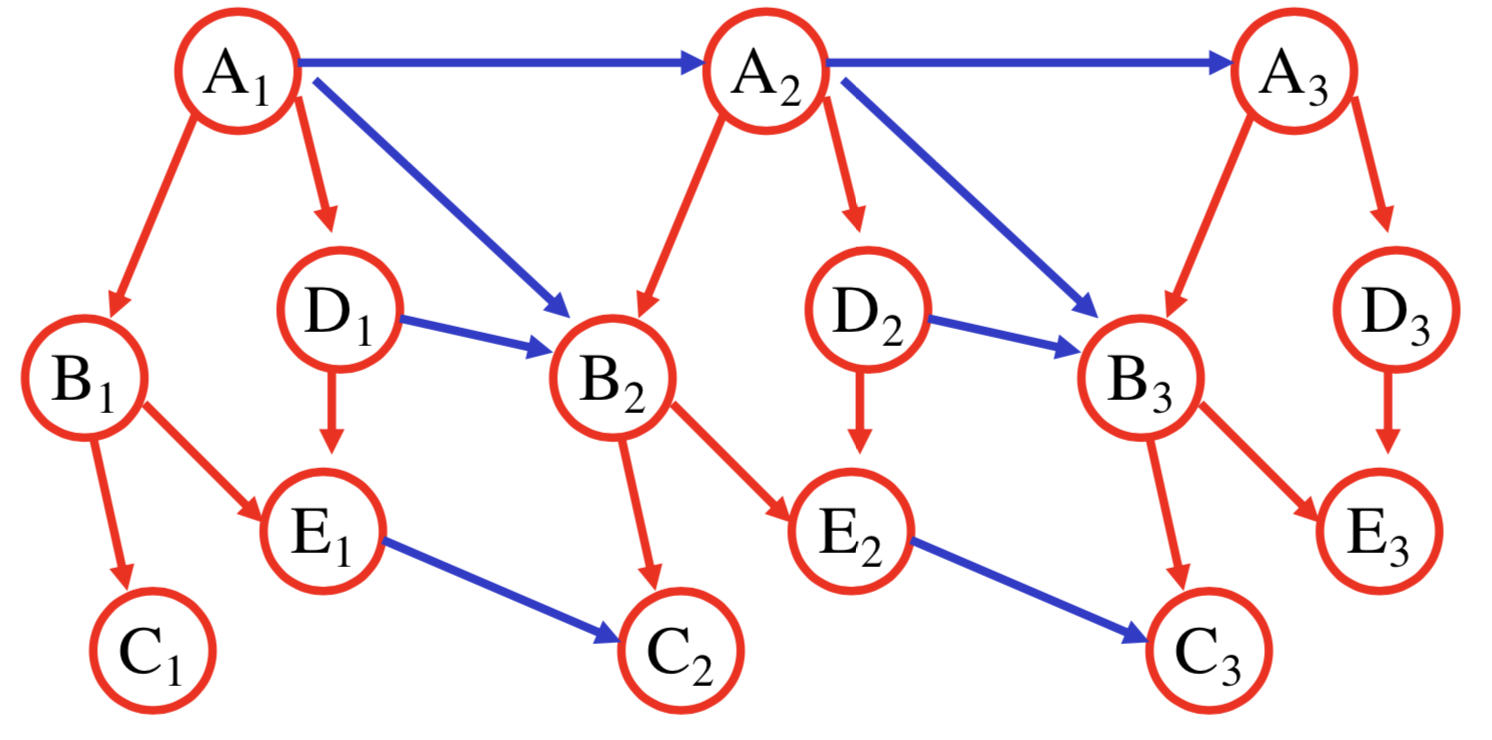
\includegraphics[scale=.1]{DBN.png}
These models typically have many loops. Exact inference is usually intractable.
\subsection{Approx. infer. for filtering (DBNs and nonlinear Kalman filters): Particle filtering}
\textbf{Suppose}: $P(X_t|y_{1:t})\approx \frac{1}{N}\sum_{i=1}^N \delta_{x_{i, t}}$, where $\delta$ is the indicator function.
\textbf{Prediction}: Propagate each particle: $x'_i \sim P(X_{t+1}|x_{i,t})$\\
\textbf{Conditioning}:\\
- weight particles $w_i=\frac{1}{Z}P(y_{t+1}|x'_i)$\\
- resample N particles $x_{i, t+1}  \sim \frac{1}{Z} \sum_{i=1}^N w_i \delta_{x'_i}$\\
% \textbf{Conclusion we came to:} $\frac{\sum_{i=1}^N w_i \delta_{x'_i}}{\sum_{i=1}^N w_i \delta_{x_i}}$
\textbf{Conclusion we came to:} $Z =\sum_{i=1}^N w_i \delta_{x_i}$

    %\section{Probabilistic Planning}
\subsection{Markov Decision Processes}
An MDP is specified by a quintuple: $(X, A, r, P(x'|x, a), \gamma)$, where $X$ are states, $A$ are actions, $r(x,a)$ is a reward function and transition probabilities:\\
    $P(x'|x,a)=\text{Prob(Next state}=x'|\text{Action } a)$\\ 
\textbf{Objective:} find a stationary policy $\pi: S \rightarrow A$ that maximizes the sum of cumulative rewards.
\textbf{Value of a state given a policy :} sum of cumulative rewards, given that the initial state is this state $\rightarrow$ \textbf{Bellman equation:}\\
$V^\pi(s)=\mathbb{E}\Big[ \sum_{t=0}^\infty \gamma^tr(s_t, \pi(s_t), s_{t+1})|s_0=s\Big]$\\
$= \sum_{s'\in S}P(s'|s, \pi(s))\big[r(s, \pi(s),s')+\gamma V^\pi(s')\big]$\\
$= r(s, \pi(s))+\gamma\sum_{s'\in S}P(s'|s,\pi(s))V^\pi(s')$

% \includegraphics[scale=0.25]{valueFunctionAndPolicy.png}
\textbf{Theorem (Bellman)}: a policy is optimal iff it is greedy w.r.t. its induced value function!\\
$V^*(x)=max_a[r(x,a)+\gamma \sum_{x'}P(x'|x,a)V^*(x')]$\\
Bellman equation mais geral: \\
$V^*(x)=max_a[ \sum_{x'}P(x'|x,a)(r(a, x, x')+\gamma V^*(x')])$
Optimal policy: \\
$\pi^*(s)=\underset{a\in A}{argmax} [r(x,a)+\gamma \sum_{x'}P(x'|x,a)V^*(x')]$

\subsection{Policy iteration (Cost $O(S^3+SA\Delta)$)}
Start with an arbitrary (e.g. random) policy $\pi$.
Until converged, do:\\
- Compute value function $V^\pi (x)$\\
- Compute greedy policy $\pi_G$ w.r.t. $V^\pi$\\
- Set $\pi \leftarrow \pi_G$\\
Guaranteed to monotonically improve and to converge to an \textbf{optimal} policy $\pi^*$ in $O(n^2m/(1-\gamma))$ iterations (converges in polynomial number of iterations)!

\subsection{Value iteration (Cost $O(SA\Delta)$)}
Initialize $V_0(x)=max_a r(x,a)$\\
For $t=1$ to $\infty$:\\
- For each $(x,a)$, let: \\
$Q_t(x,a)=r(x,a)+\gamma\sum_{x'}P(x'|x,a)V_{t-1}(x')$\\
- For each $x$, let $V_t(x)=\underset{a}{max}Q_t(x,a)$\\
- Break if $||V_t-V_{t-1}||_{\infty}=\underset{x}{max}|V_t(x)-V_{t-1}(x)|\leq\epsilon$\\
Then choose greedy policy w.r.t $V_t$.\\
Guaranteed to converge to $\epsilon$-optimal policy (finds approximate solution in polynomial number of iterations)!

\subsection{POMDP = Belief-state MDP}
States = beliefs over states for original POMDP\\
$B=\Delta({1,...,n})=\{ b:{1,...,n} \rightarrow [0,1],\sum_x b(x)=1 \}$\\
Actions: same as original MDP\\
\textbf{Transition model:}\\
- Stochastic observation:\\
$P(Y_t|b_t)=\sum_{x=1}^n P(Y_t|X_t=x)b_t(x)$\\
- State update (Bayesian filtering!), given $b_t, y_t, a_t$:
$b_{t+1}(x')=\frac{1}{Z}\sum_xb_t(x)P(y_t|x)P(X_{t+1}=x'|X_t=x,a_t)$\\
Reward function: $r(b_t, a_t)=\sum_x b_t(x)r(x,a_t)$

\subsection{Example of approx. solution to POMDPs: Policy gradients}
- Assume parameterized policy: $\pi(b)=\pi(b;\theta)$\\
- For each parameter $\theta$ the policy induces a Markov chain\\
- Can compute expected reward $J(\theta)$ by sampling.\\
- Find optimal parameters through search (gradient ascent):
$\theta^* = \underset{\theta}{arg max}\quad J(\theta)$



    %\section{Learning models from training data}
\subsection{Learning from i.i.d data}
\textbf{Algorithm for Bayes Net MLE}:\\
Given BN of structure G and dataset D of complete observations\\
For each $X_i$ estimate:
$\hat{\theta}_{X_i|Pa_i}=\frac{Count(X_i, Pa_i)}{Count(Pa_i)}$\\
Pseudo-counts for lime and cherry flavor: $\theta_{F=c}\frac{Count(F=c)+\alpha_c}{N+\alpha_c + \alpha_l}$

\subsubsection{Score based structure learning}
Define scoring function $S(G;D)$ and search over BN structure G: $G^*=\underset{G}{argmax}S(G;D)$\\
\textbf{Examples of scores:\\
MLE Score}:\\
$log P(D|\theta_G, G) = N \sum_{i=1}^n \hat{I}(X_i;Pa_i) + const.$\\
\textbf{Where mutual information} ($I(X_i, X_j)\geq 0$) is:\\
$I(X_i, X_j)=\sum_{x_i, x_j}P(x_i, x_j)log\frac{P(x_i, x_j)}{P(x_i)P(x_j)}$ \\
\textbf{Empirical mutual information:}\\
$\hat{P}(x_i,x_j)=\frac{Count(x_i, x_j)}{N}$\\
$\hat{I}(X_i, X_j)= \sum_{x_i, x_j}\hat{P}(x_i, x_j)log\frac{\hat{P}(x_i, x_j)}{\hat{P}(x_i)\hat{P}(x_j)}$\\
\textbf{Regularizing a Bayes Net:}\\
$S_{BIC}(G) = \sum_{i=1}^n \hat{I}(X_i;Pa_i) - \frac{log N}{2N}|G|$ \\
where $G$ is the number of parameters, $n$ the number of variables and $N$ the number of training examples.\\
\textbf{Chow-Liu algorithm:}\\
- For each pair $X_i, X_j$ of variables, compute: $\hat{P}(x_i,x_j)=\frac{Count(x_i, x_j)}{N}$\\
- Compute mutual information\\
- Define complete graph with weight of edge $(X_i, X_j)$ given by the mutual information\\
- Find max spanning tree $\rightarrow$ undirected tree\\
- Pick any variable as root and orient the edges away using breadth-first search.\\


    \section{Non Parametric RL}
It is an MDP with unknown $p(x'\vert x,a)$ and $r(x,a)$

\subsection{Model-based RL}
From all steps $X_{t+1},R_t \vert X_{t}, A_{t}$ we can learn:\\
$p(x'\vert x,a)\simeq \hat{p}_{x'\vert x, a} = \frac{Count(X_{t+1}=x',\; X_t=x,\;A_t =a)}{Count(X_t=x,\; A_t = a)}$\\
$r(x,a)\simeq \hat{r}_{x,a}= \frac{1}{Count(X_t=x,\; A_t=a)}\sum_{t|X_t=x,\; A_t=a}R_t$\\
How to chose $a_t$?

\subsubsection{$\epsilon$-greedy (On-Policy)}
With probability $\epsilon$, pick random action.\\
With probability $1-\epsilon$, pick $a = \argmax Q(x,a)$.\\
\textbf{Oss:} $Q$ is caclulated from $(\hat{p}, \hat{r})$\\
\textbf{Th:} If $\epsilon_t\xrightarrow{RM}0$ then $(\hat{r},\hat{p})\xrightarrow{a.s.}(r,p)$

\subsubsection{Softmax (On-Policy)}
Draw $a \sim q(a\vert x) = \text{softmax}\frac{Q(x,a)}{\tau}$\\
If $\tau \uparrow $ it means I trust less $Q$

\subsubsection{$R_{max}$ algorithm (On-Policy)}
We add a fairy state $x^*$\\
\begin{algorithm}[H]
    \SetKwInput{kwInit}{init}
    \kwInit{$r(x,a) = R_{max} \; \forall x\in \mathcal{X}\cup \left\{x^*\right\},a\in\mathcal{A}$}
    \kwInit{$p(x^*\vert x, a) = 1 \; \forall x\in \mathcal{X},a\in\mathcal{A}$}
    \kwInit{$\pi = $ optimal policy w.r.t. $p$, $r$}
    \Repeat{}{  
        Execute $\pi$ and get $x_{t+1}$ and $r_t$\\
        Update belief of $r(x_t,\pi(x_t))$ and $p(x_{t+1}\vert x_t,\pi(x_t))$\\
        If obeserved 'enough' in $(x,a)$ recompute $\pi$ using the updated belief only in $(x,a)$
    }
\end{algorithm}
\textbf{'Enough'?} See Hoeffding's inequality \\
($\hat{p}\in [0, 1],\; \hat{r}\in [0, R_{max}]$).\\
\textbf{PAC bound:} With probability $1-\delta$, $R_{max}$ will reach an $\epsilon$-optimal policy in a number of steps that is polynomial in $|X|, |A|, T, 1/\epsilon$ and $log(1/\delta)$. Memory $O(|X|^2|A|)$. 

\subsection{Model-free RL}
Learn $\pi^*$ only via $V^*$ or $Q^{V^*}$

\subsubsection{TD-learning (On-Policy)}
Given a policy $\pi$ we want to learn $V^\pi$\\
$V^\pi(x)=\mathbb{E}_{R\sim r(x,\pi(x)), X'\sim p(\cdot\vert x, \pi(x))}\left[R + \gamma V^\pi(X')\right]$\\
After seeing $(x_{t+1}, r_t \vert x_t, \pi(x_t))$ we update: \\
$V_{t+1}(x_t)\gets (1-\alpha_t)V_{t}(x_t) + \alpha_t(r_t + \gamma V_t^\pi(x_{t+1}))$\\
Where $\alpha_t$ is a regulizer term (only 1 samlple)
\textbf{Th:} If $\alpha_t\xrightarrow{RM}0$ then $V\xrightarrow{a.s.}V^\pi$

\subsubsection{Q-learning (Off Policy)}
Given experience we want to learn $Q^* = Q^{V^*}$\\
$Q^*(x,a) = \mathbb{E}_{\substack{R\sim r(x,\pi(x)) \\ X'\sim p(\cdot\vert x, \pi(x))}}\left[R+\gamma \max_{a'} Q^*(X',a')\right]$\\
After seeing $(x_{t+1}, r_t \vert x_t, a_t)$ we update: \\
$Q(x_t,a_t) ${\scriptsize $\gets (1-\alpha_t)Q(x_t,a_t) + \alpha_t(r_t+\gamma \max_{a'}Q(x_{t+1}, a'))$}\\
% $V^*(x)=\underset{a}{max}Q*(x,a)$\\
\textbf{Th:} If $\alpha_t\xrightarrow{RM}0$ then $Q\xrightarrow{a.s.}Q^{*}$\\
\textbf{Optimistic Q learning:}\\
Initialize: $Q(x,a)=\frac{R_{max}}{1-\gamma}\prod_{t=1}^{T_{init}}(1-\alpha_t)^{-1}$\\
Same convergence time as with $R_{max}$. Memory $O(|X||A|)$. Comp: $O(|A|)$.

\section{Parametric RL}
\subsection{Parametric TD-learning}
\subsubsection{TD-learinging as SGD}
TD-learing = 1 sample ($x', r \vert x, \pi(x)$) SGD on:\\
$\bar{l}_2(V;x,r) = \frac{1}{2}\left(V-r-\gamma\mathbb{E}_{x'\sim p(\cdot\vert x, \pi(x))}\left[\hat{V}^\pi(x')\right]\right)^2$\\
1 sample estimate of $\nabla_V \bar{l}_2 = \delta = V-r-\gamma \hat{V}^\pi(x')$\\
$\Rightarrow V\gets V - \alpha_t \delta$ where $V = \hat{V}^\pi(x)$

\subsubsection{TD-parametric}
If $\hat{V}^\pi(x) = V(x,\theta)$ then: \\
$\delta = \left[ V(x;\theta)-r-\gamma V(x';\theta_{old})\right] \nabla_\theta V(x,\theta)$

\subsection{Parametric Q-learining}
$\delta (\theta, \theta_{old}) = \left(Q(x,a;\theta)-r-\gamma\max_{a'} Q(x',a';\theta_{old})\right)$\\
We don't differiantiate with regard to $\theta_{old}$\\
The SGD step is:
$\theta \gets \theta - \alpha_t \delta(\theta, \theta) \nabla_\theta Q(x,a;\theta)$

\textbf{Deep Q Networks (DQN):} Version of Q-learning where we update $Q$ only each batch:\\
{\scriptsize $L(\theta) = \sum_{(x,a,r,x')\in\mathcal{D}}\left(r+\gamma\max_{a'}Q(x',a';\theta_{old})-Q(x,a;\theta)\right)^2$}
\textbf{Double DQN (better):} \\
{\scriptsize $L(\theta) = \sum_{(x,a,r,x')\in\mathcal{D}}\left(r+\gamma Q(x',a^*(\theta);\theta_{old})-Q(x,a;\theta)\right)^2$}\\
where: $a^*(\theta) \doteq \argmax_{a'}Q(x',a'; \theta)$\\
\subsection{Policy-Search method}




\end{multicols*}
\end{document}